%%%%%%%%%%%%%%%%%%%%%%%%%%%%%%%%%%%%%%%%%
% Beamer Presentation
% LaTeX Template
% Version 1.0 (10/11/12)
%
% This template has been downloaded from:
% http://www.LaTeXTemplates.com
%
% License:
% CC BY-NC-SA 3.0 (http://creativecommons.org/licenses/by-nc-sa/3.0/)
%
%%%%%%%%%%%%%%%%%%%%%%%%%%%%%%%%%%%%%%%%%

%----------------------------------------------------------------------------------------
% PACKAGES AND THEMES
%----------------------------------------------------------------------------------------

\documentclass[10pt,xcolor={dvipsnames}]{beamer}
%\setbeamersize{text margin left=1em,text margin right=1em}
\usepackage{mathtools}
\usepackage{amsmath}
\usepackage{bm}
\usepackage{hyperref}

\usepackage{graphicx} % Allows including images
\graphicspath{{/Users/rebecca/Documents/Rivet_Analyses/MC_VBFDM/PlotCombinationTool/Figures/}{/Users/rebecca/Documents/Presentations/Talks/}}
\usepackage{booktabs} % Allows the use of \toprule, \midrule and \bottomrule in tables

\usepackage{etoolbox}

\usepackage{subcaption}
\captionsetup{compatibility=false}

\usepackage{multirow}

\usepackage{appendixnumberbeamer}
\usepackage{cancel}
%\newlength\origleftmargini
%\setlength\origleftmargini\leftmargini
%\setbeamertemplate{itemize/enumerate body begin}{\setlength{\leftmargini}{2pt}}%

%\let\oldexampleblock\exampleblock
%\let\oldendexampleblock\endexampleblock
%\def\exampleblock{\begingroup \setbeamertemplate{itemize/enumerate body begin}{\setlength{\leftmargini}{\origleftmargini}} \oldexampleblock}
%\def\endexampleblock{\oldendexampleblock \endgroup}%

%\let\oldalertblock\alertblock
%\let\oldendalertblock\endalertblock
%\def\alertblock{\begingroup \setbeamertemplate{itemize/enumerate body begin}{\setlength{\leftmargini}{\origleftmargini}} \oldalertblock}
%\def\endalertblock{\oldendalertblock \endgroup}

\mode<presentation> {

% The Beamer class comes with a number of default slide themes
% which change the colors and layouts of slides. Below this is a list
% of all the themes, uncomment each in turn to see what they look like.

%\usetheme{default}
%\usetheme{AnnArbor}
%\usetheme{Antibes}
%\usetheme{Bergen}
%\usetheme{Berkeley}
%\usetheme{Berlin}
\usetheme{Boadilla}
%\usetheme{CambridgeUS}
%\usetheme{Copenhagen}
%\usetheme{Darmstadt}
%\usetheme{Dresden}
%\usetheme{Frankfurt}
%\usetheme{Goettingen}
%\usetheme{Hannover}
%\usetheme{Ilmenau}
%\usetheme{JuanLesPins}
%\usetheme{Luebeck}
%\usetheme{Madrid}
%\usetheme{Malmoe}
%\usetheme{Marburg}
%\usetheme{Montpellier}
%\usetheme{PaloAlto}
%\usetheme{Pittsburgh}
%\usetheme{Rochester}
%\usetheme{Seahorse}
%\usetheme{Singapore}
%\usetheme{Szeged}
%\usetheme{Warsaw}

% As well as themes, the Beamer class has a number of color themes
% for any slide theme. Uncomment each of these in turn to see how it
% changes the colors of your current slide theme.

%\usecolortheme{albatross}
%\usecolortheme{beaver}
%\usecolortheme{beetle}
%\usecolortheme{crane}
%\usecolortheme{dolphin}
%\usecolortheme{dove}
%\usecolortheme{fly}
%\usecolortheme{lily}
%\usecolortheme{RoyalBlue}
%\usecolortheme{rose}
%\usecolortheme{seagull}
%\usecolortheme{seahorse}
%\usecolortheme{whale}
%\usecolortheme{wolverine}

%%Changing the theme colours
%\setbeamercolor*{structure}{bg=Plum!20,fg=Plum}
%\setbeamercolor*{palette primary}{use=structure,fg=white,bg=structure.fg}
%\setbeamercolor*{palette secondary}{use=structure,fg=white,bg=structure.fg!75}
%\setbeamercolor*{palette tertiary}{use=structure,fg=white,bg=structure.fg!50!black}
%\setbeamercolor*{palette quaternary}{fg=white,bg=black}
%\setbeamercolor{section in toc}{fg=black,bg=white}
%%\setbeamercolor{alerted text}{use=structure,fg=structure.fg!50!black!80!black}
%\setbeamercolor{titlelike}{parent=palette primary,fg=structure.fg!50!black}
%\setbeamercolor{frametitle}{bg=gray!30!white,fg=Plum}
%\setbeamercolor*{titlelike}{parent=palette primary}

%Changing the theme colours
\setbeamercolor*{structure}{bg=RoyalPurple,fg=RoyalPurple}
\setbeamercolor*{palette primary}{use=structure,fg=white,bg=structure.fg}
\setbeamercolor*{palette secondary}{use=structure,fg=white,bg=structure.fg}
\setbeamercolor*{palette tertiary}{use=structure,fg=white,bg=structure.fg}
\setbeamercolor*{palette quaternary}{fg=white,bg=black}
\setbeamercolor{section in toc}{fg=black,bg=white}
%\setbeamercolor{alerted text}{use=structure,fg=structure.fg!50!black!80!black}
\setbeamercolor{titlelike}{parent=palette primary,fg=structure.fg!50!black}
%\setbeamercolor{frametitle}{use=structure,fg=white,bg=structure.fg}
\setbeamercolor*{titlelike}{parent=palette primary}

%\setbeamercolor{block}{bg=yellow!10,fg=black}
%\setbeamercolor{block title}{bg=yellow!50,fg=black}
%\AtBeginEnvironment{block}{\setbeamercolor{itemize item}{fg=yellow}}

\newenvironment<>{examplefirst}[1]{%
  \setbeamercolor{block title}{bg=yellow!50,fg=black}%
  \begin{block}#2{#1}}{\end{block}}
\AtBeginEnvironment{examplefirst}{\setbeamercolor{itemize item}{fg=yellow}}

%\setbeamertemplate{footline} % To remove the footer line in all slides uncomment this line
%\setbeamertemplate{footline}[page number] % To replace the footer line in all slides with a simple slide count uncomment this line

%\setbeamertemplate{navigation symbols}{} % To remove the navigation symbols from the bottom of all slides uncomment this line


\setbeamertemplate{blocks}[rounded][shadow=false]
\setbeamertemplate{itemize items}[circle]
\setbeamertemplate{itemize subitems}[circle]

\renewcommand{\thefootnote}{\alph{footnote}}

}

%----------------------------------------------------------------------------------------
% TITLE PAGE
%----------------------------------------------------------------------------------------



\title[Christmas Meeting Talk]{Climbing, Dark Matter and the Resolution of Jet Energy.} % The short title appears at the bottom of every slide, the full title is only on the title page

\author{\underline{Rebecca Pickles}} % Your name
%\institute[UoM] % Your institution as it will appear on the bottom of every slide, may be shorthand to save space
%{
%University of Manchester\\ % Your institution for the title page
%\medskip
%\textit{julia.iturbe@cern.ch} % Your email address
%}
% logo of my university
\titlegraphic{
\includegraphics[width=3cm]{UniOfManchesterLogo}}
\date{December 21, 2015} % Date, can be changed to a custom date

\begin{document}

\begin{frame}
\titlepage % Print the title page as the first slide
\end{frame}

\iffalse
\begin{frame}
\frametitle{Overview} % Table of contents slide, comment this block out to remove it
\tableofcontents % Throughout your presentation, if you choose to use \section{} and \subsection{} commands, these will automatically be printed on this slide as an overview of your presentation
\end{frame}
\fi
%----------------------------------------------------------------------------------------
% PRESENTATION SLIDES
%----------------------------------------------------------------------------------------

%------------------------------------------------
\section{Introduction} % Sections can be created in order to organize your presentation into discrete blocks, all sections and subsections are automatically printed in the table of contents as an overview of the talk

%------------------------------------------------
\iffalse
\fi


\begin{frame}
\frametitle{A bit about me:}
\begin{itemize}
\item First year PhD student (Started in September)
\item Completed my Undergraduate degree here at Manchester.
\item MPhys Project was on DUNE.
\end{itemize}
\end{frame}

\begin{frame}
\frametitle{Non-academic / Climbing:}
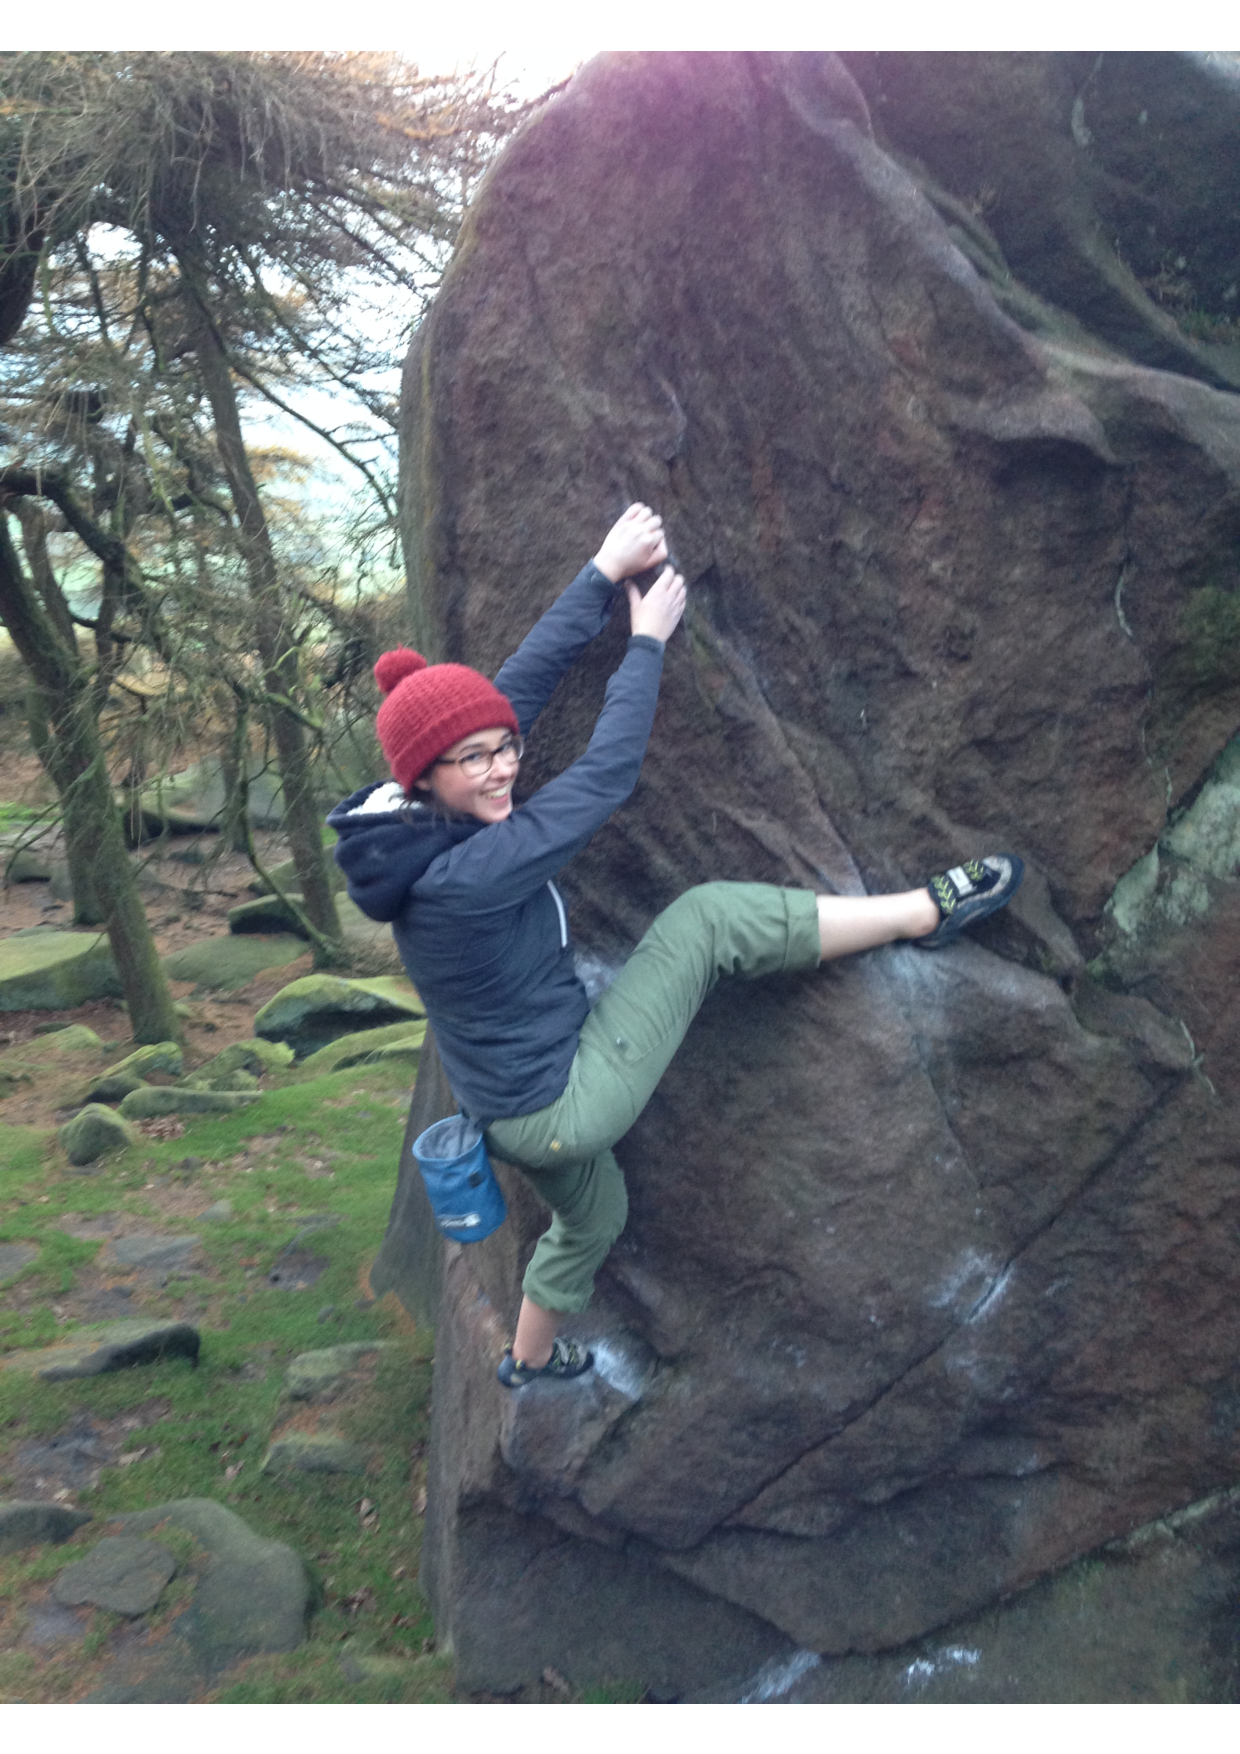
\includegraphics[width=2cm]{climbingpic1}
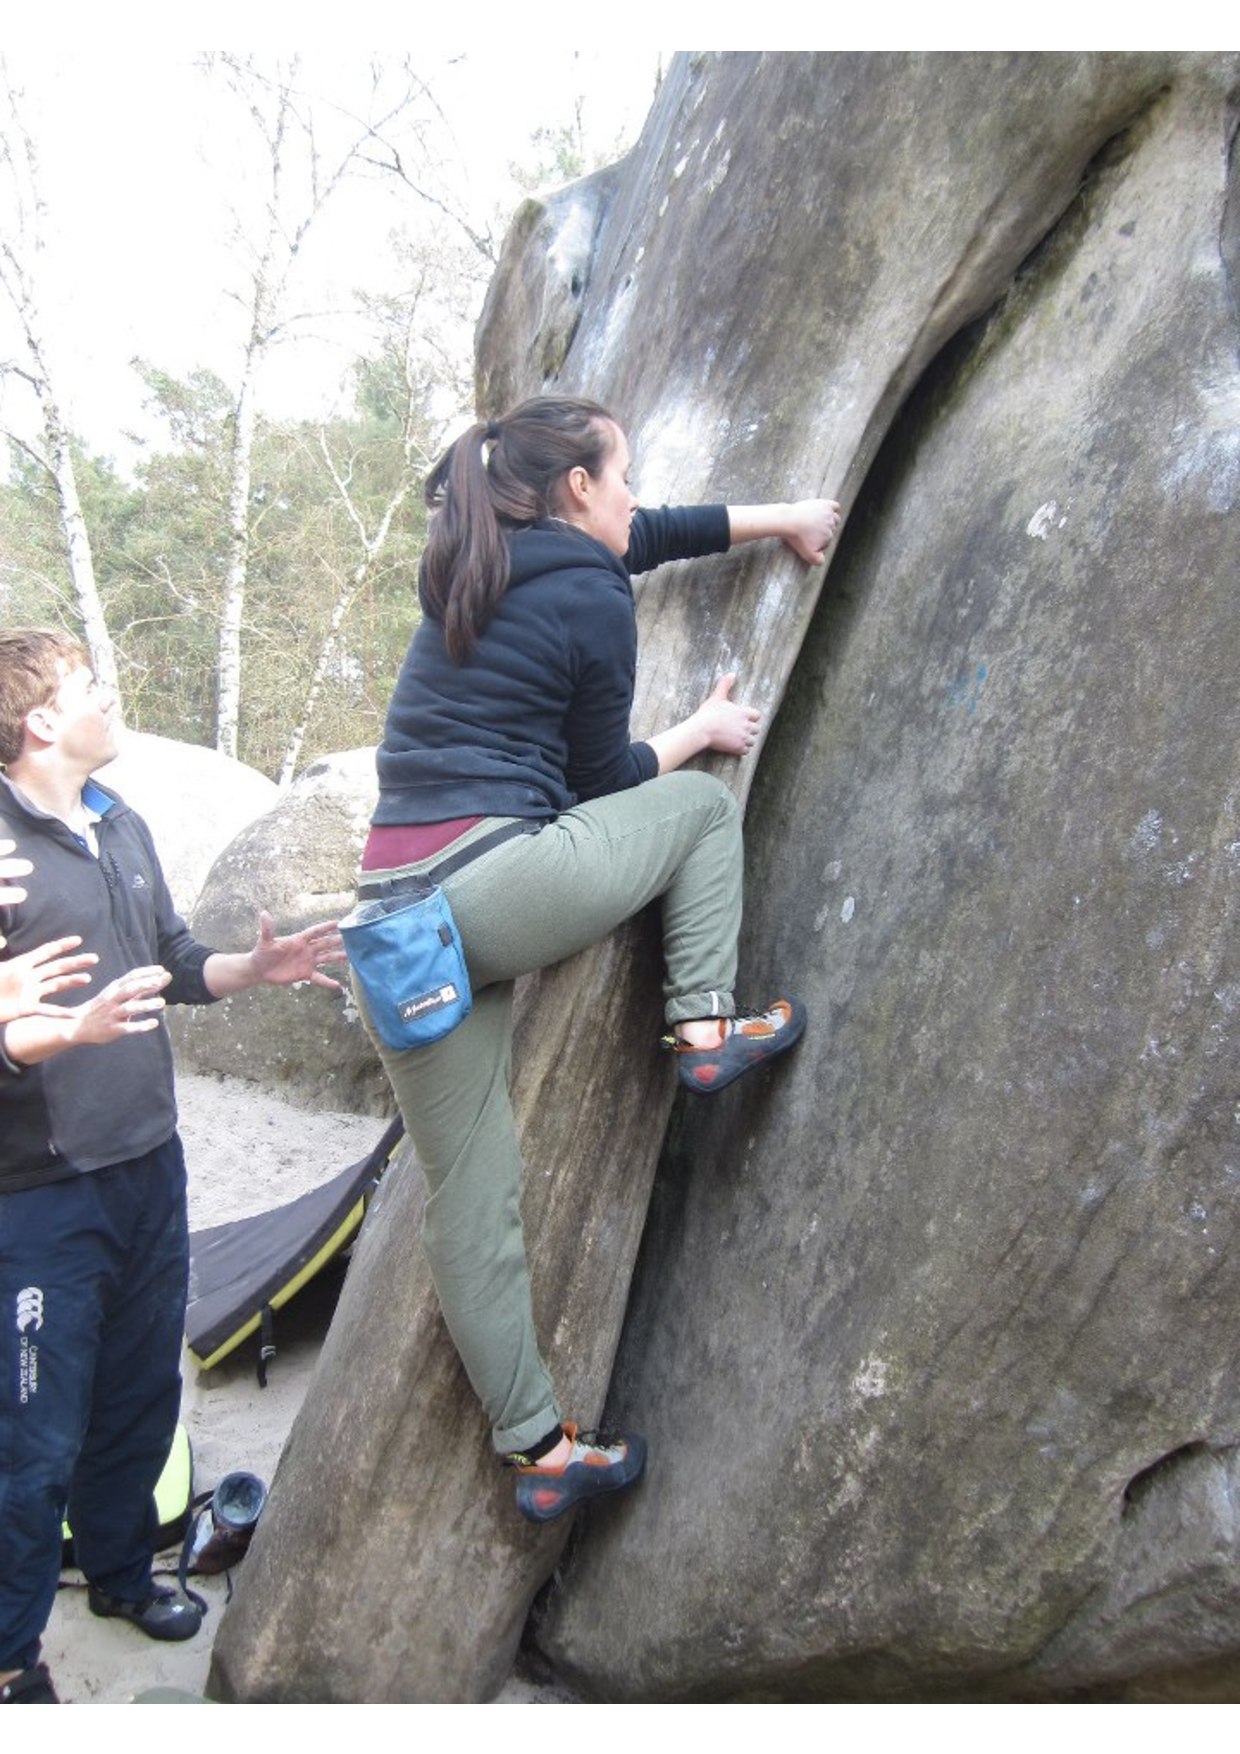
\includegraphics[width=2cm]{climbingpic6}
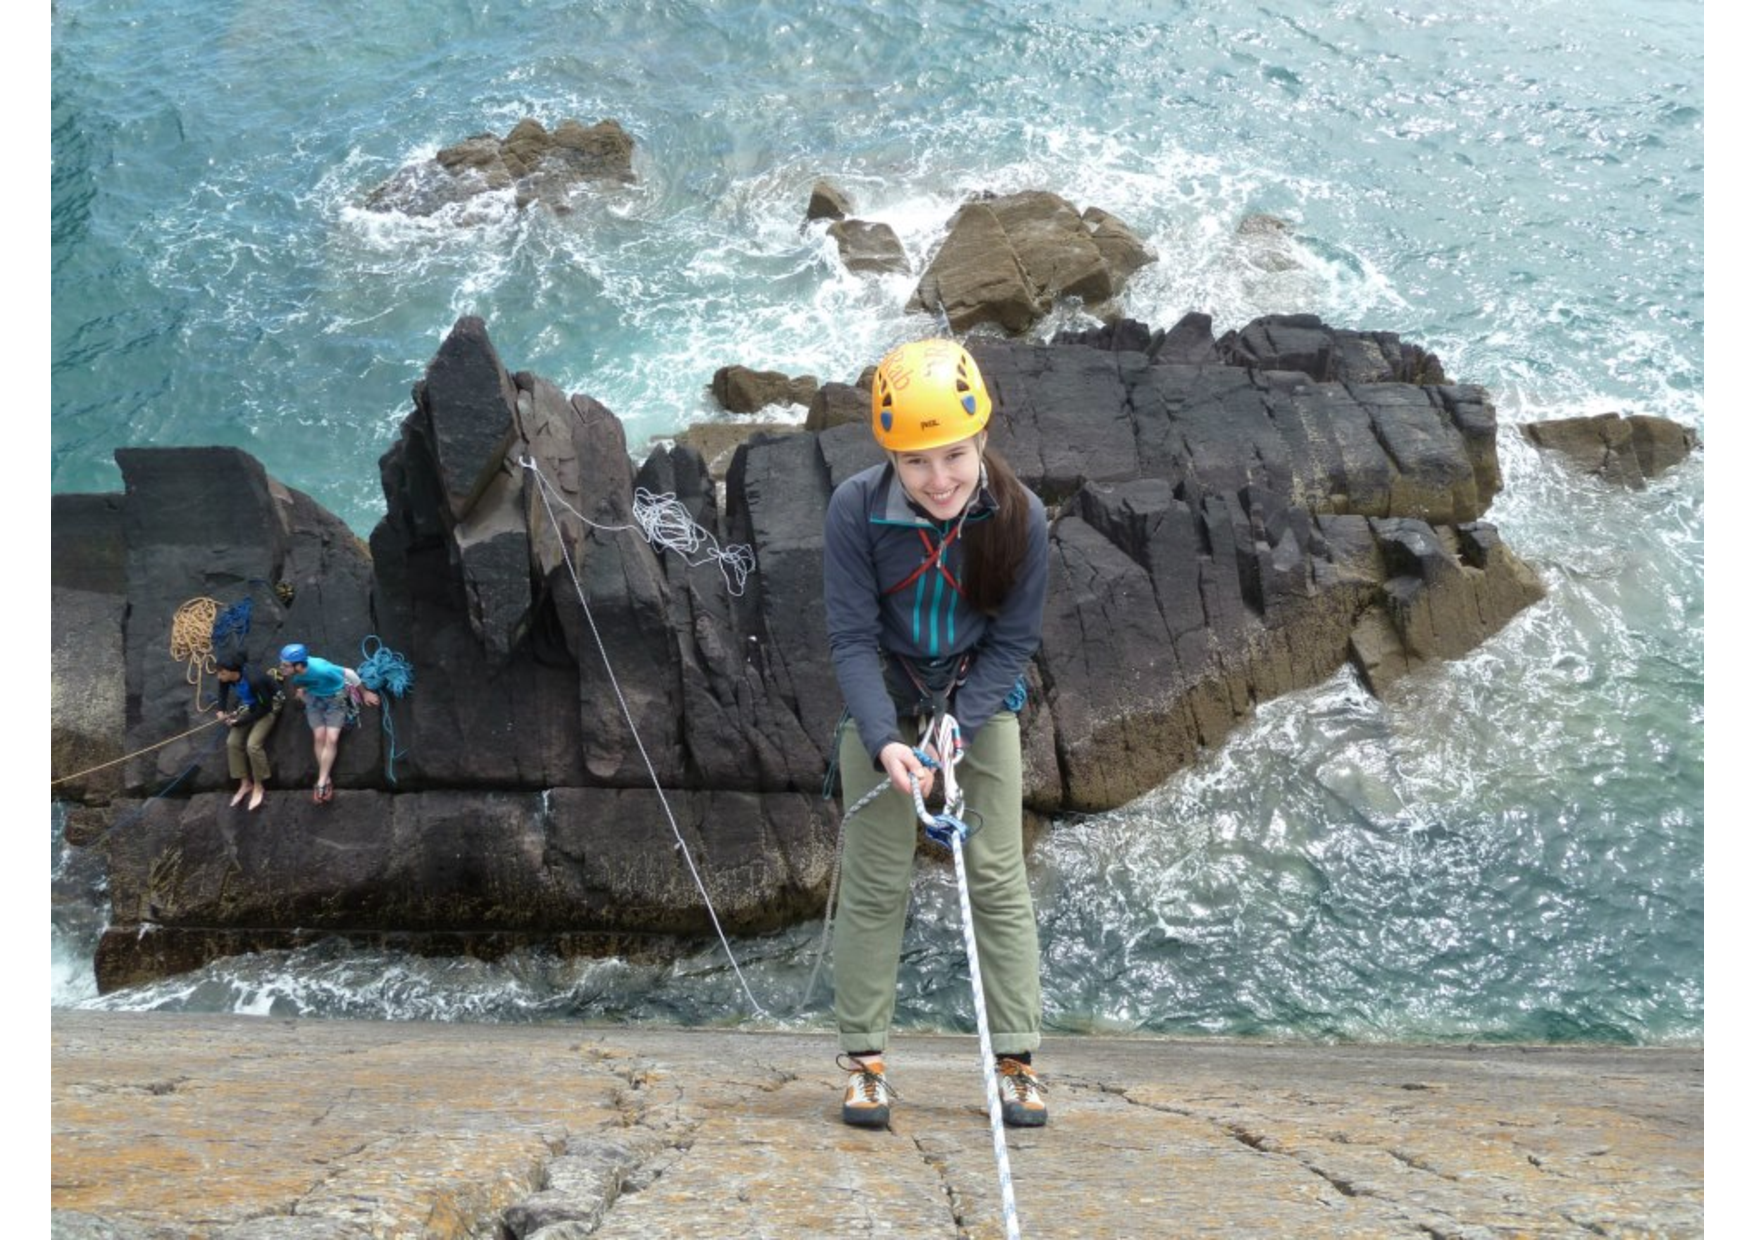
\includegraphics[width=4cm]{climbingpic5}
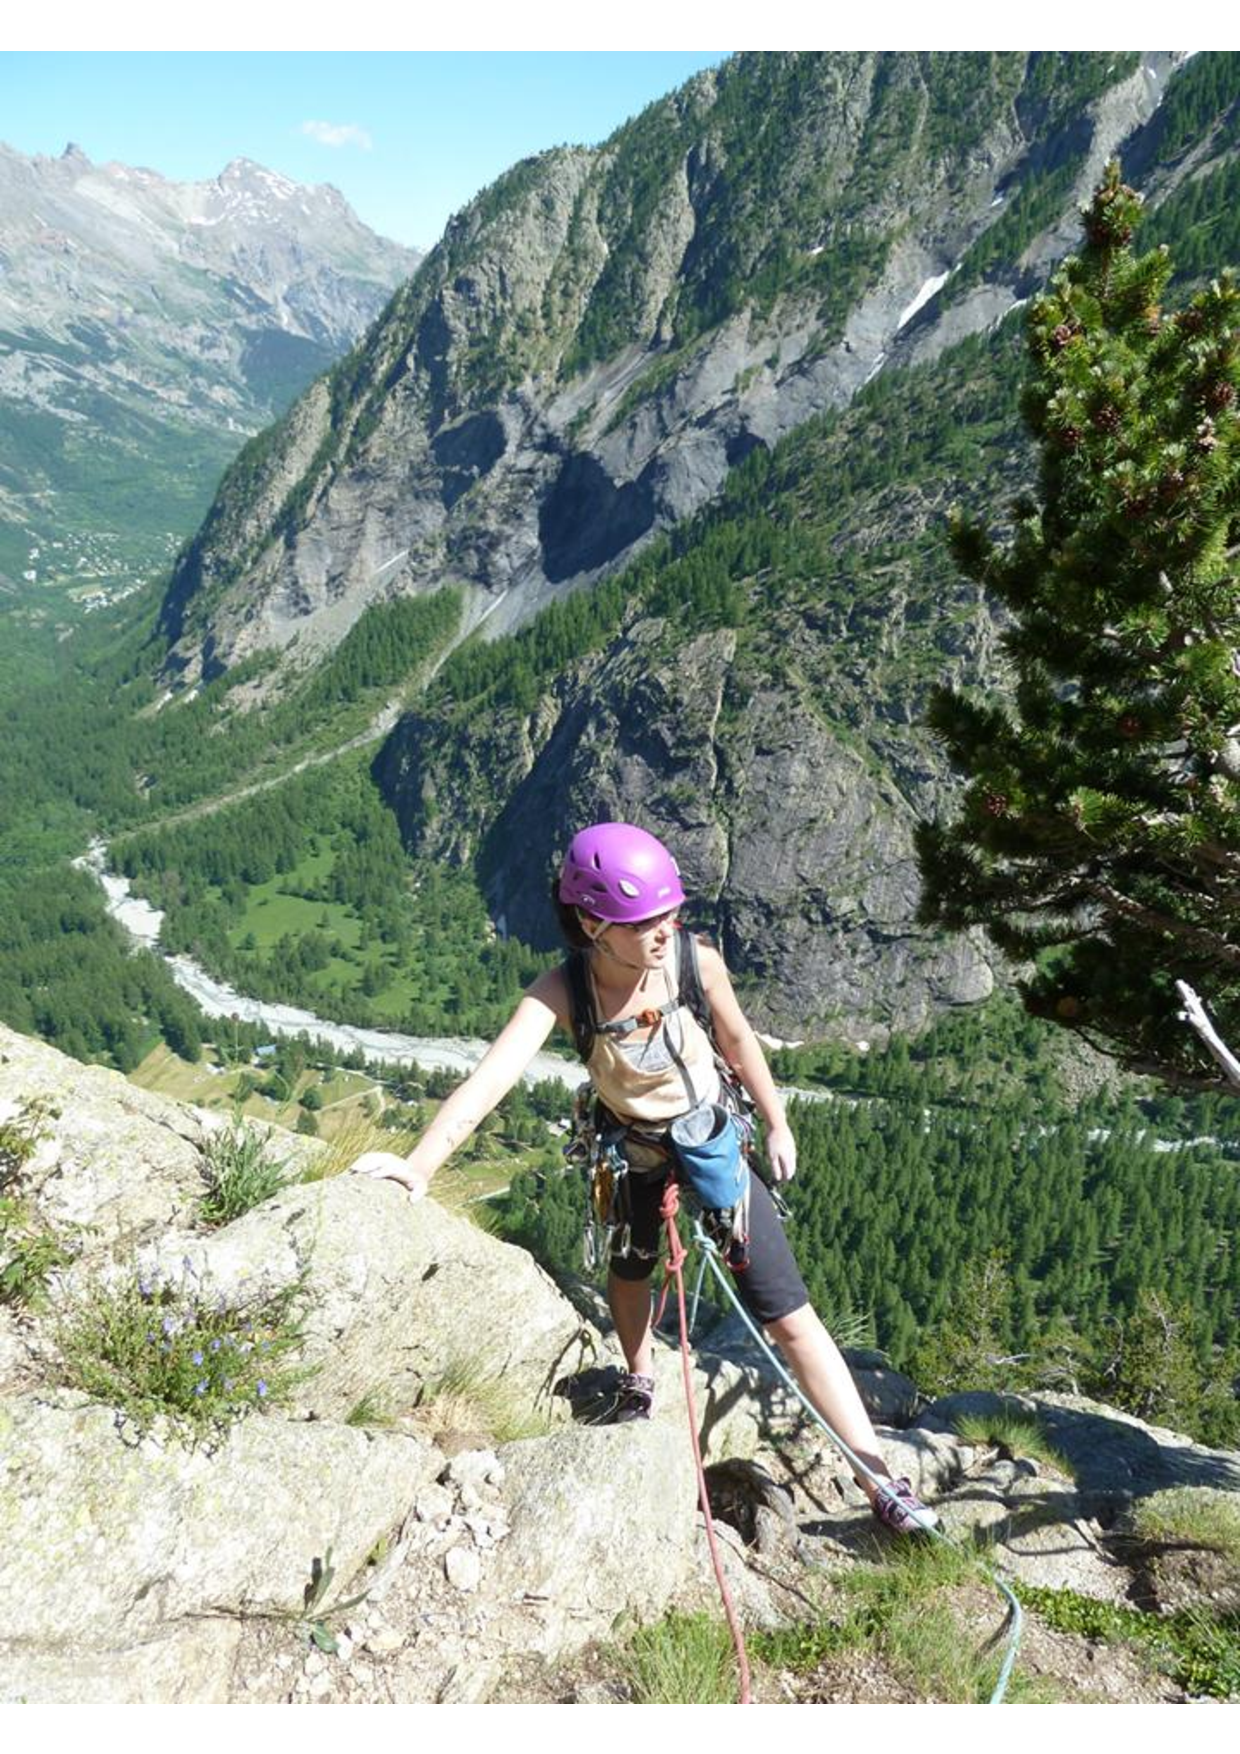
\includegraphics[width=2cm]{climbingpic3}
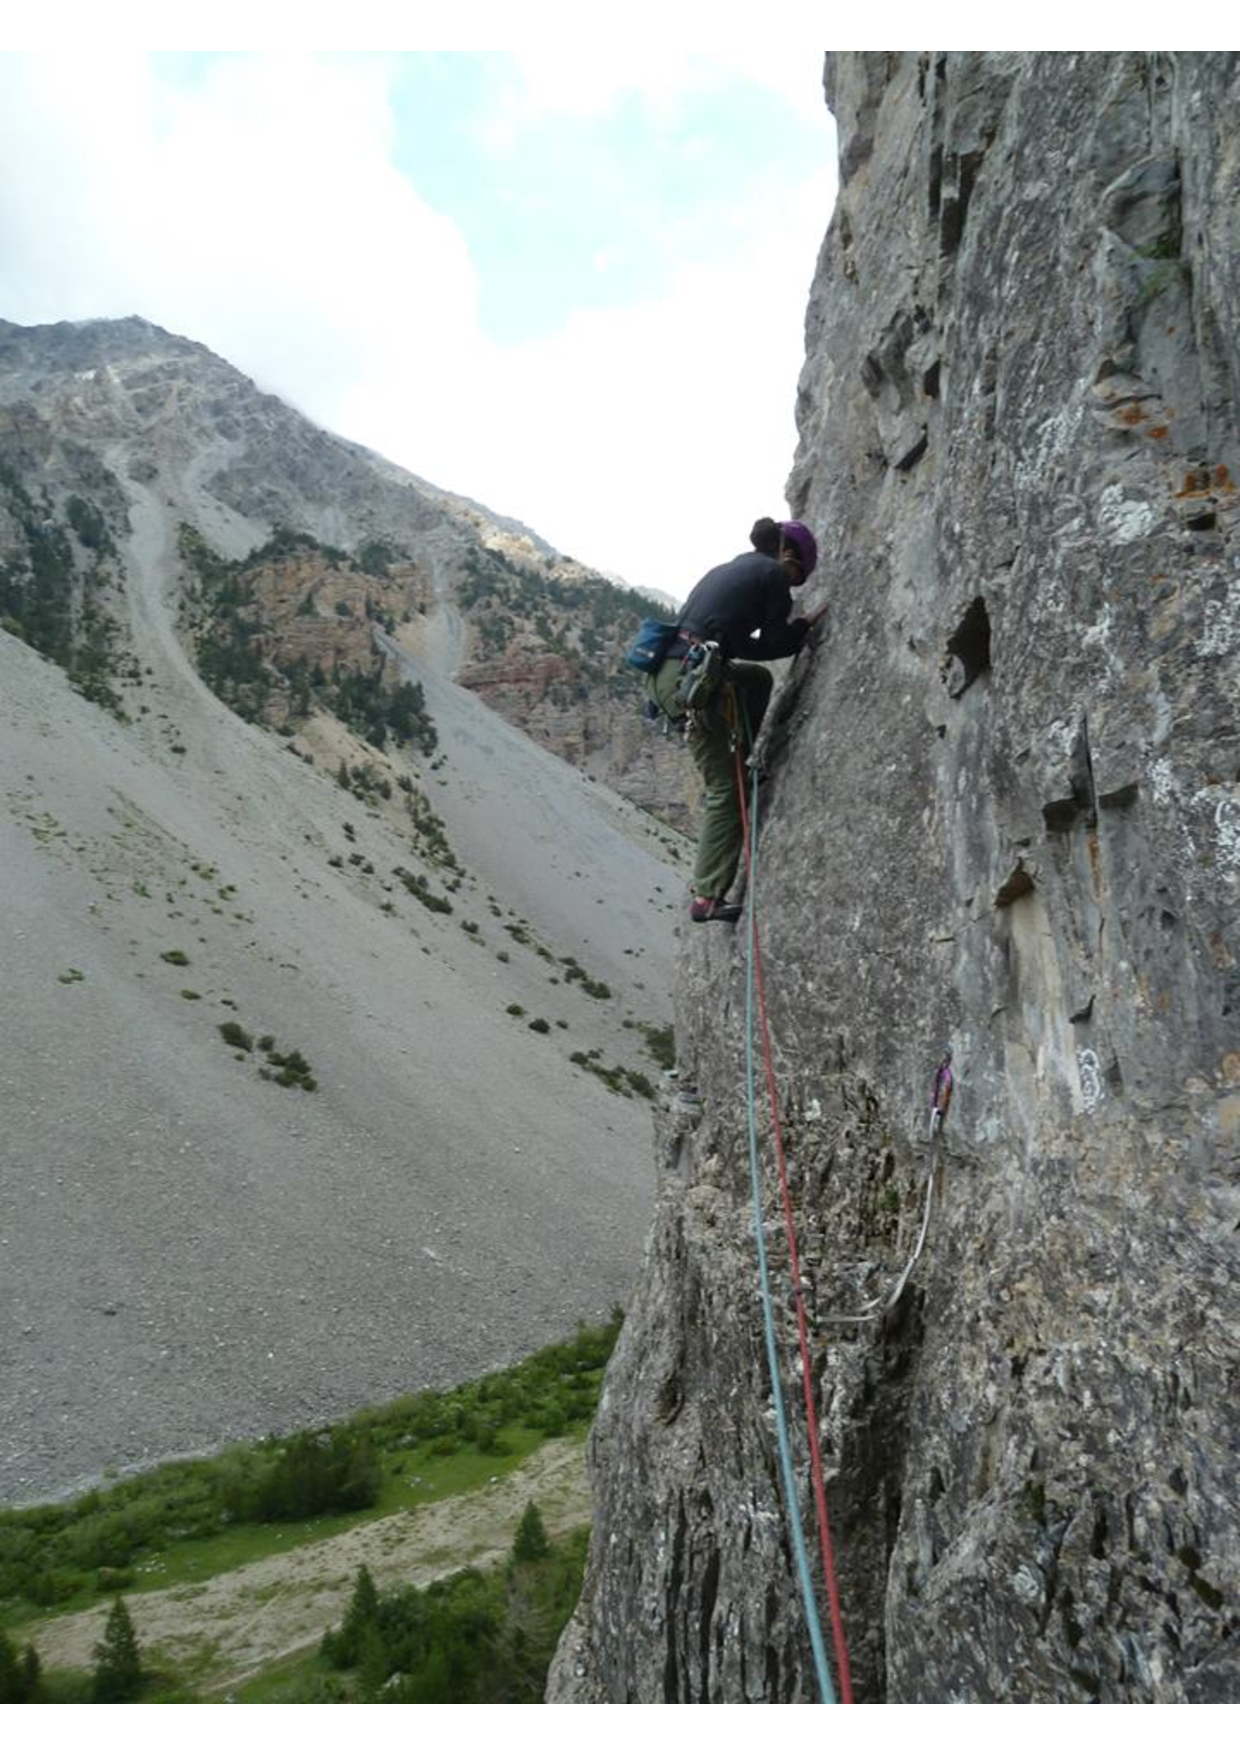
\includegraphics[width=2cm]{climbingpic4}

\center{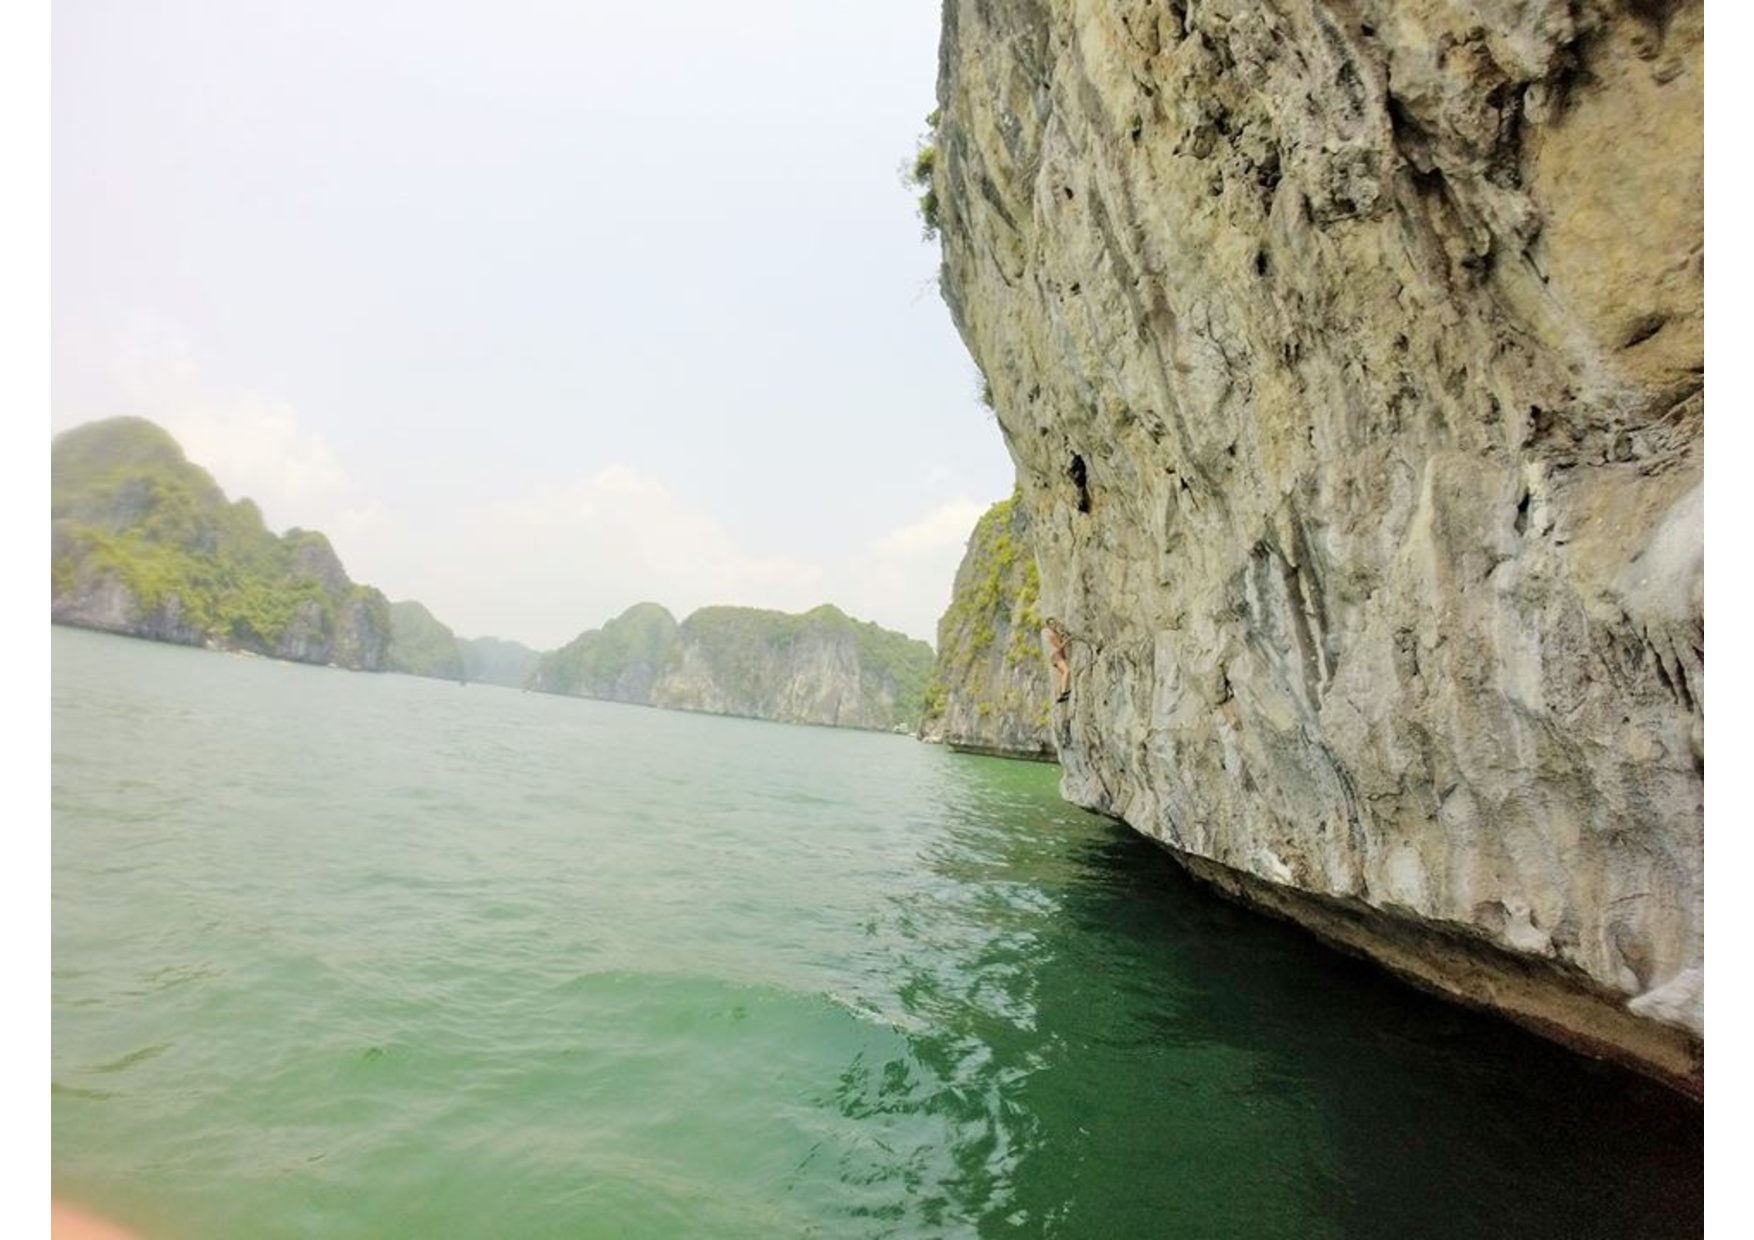
\includegraphics[width=7cm]{climbingpic12}}
\end{frame}

\begin{frame}
\frametitle{Vector Boson Fusion Dark Matter Models}
Using weak boson fusion as a mechanism for the production of exotic particles, such as dark matter and neutrinos at the ATLAS experiment at the LHC.
\newline
\begin{columns}
\begin{column}{.6\textwidth}
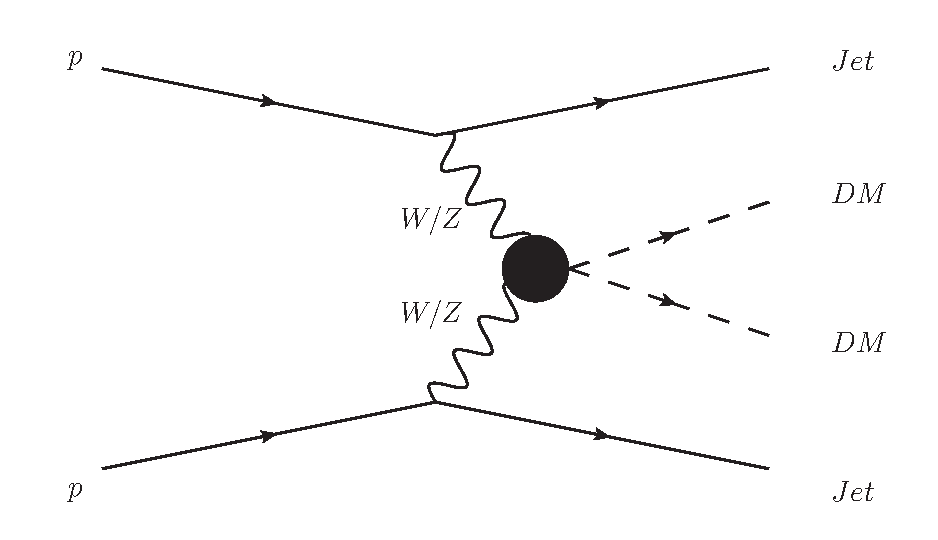
\includegraphics[width=7cm]{ppdmdmjj_feynman}
\end{column}
\begin{column}{.4\textwidth}
\begin{exampleblock}{Dark Matter Models}
\begin{itemize}
\item Looking at effective field theories to produce models of DM events in the ATLAS detector.
\item Using and analysing these generated DM events to establish sensitivity.
\end{itemize}
\end{exampleblock}
\end{column}
\end{columns}
\begin{block}{Long Term Plan:}
\begin{itemize}
\item Use this mechanism to look for the origin of the neutrino mass and other electroweak phenomena.
\end{itemize}
\end{block}

\end{frame}

\begin{frame}
\frametitle{DM Plot Examples}
\begin{columns}
\begin{column}{.5\textwidth}
\center{$\cancel{E}_{T}$}
\includegraphics[width=6cm, height=7cm]{/Mass10/Absolute/Mass10_ETMiss_PS_VBFDM.pdf}
\end{column}
\begin{column}{.5\textwidth}
\center{$\Delta\eta$}
\includegraphics[width=6cm, height=7cm]{/Mass10/Absolute/Mass10_DeltaEta_PS_VBFDM.pdf}
\end{column}
\end{columns}
\end{frame}

\begin{frame}
\frametitle{Qualifiation Task: Jet Energy Resolution}
Determining the jet resolution from data to make precise jet measurements.
\begin{block}{This measurement is vital for:}
\begin{itemize}
\item The measurement of the cross-sections of Jets, dijets, mulitjets and vector bosons accompanied by jets.
\item Top-quark cross-sections and mass measurements.
\item Determination of missing transverse energy.
\end{itemize}
\end{block}
\begin{columns}
\begin{column}{.5\textwidth}
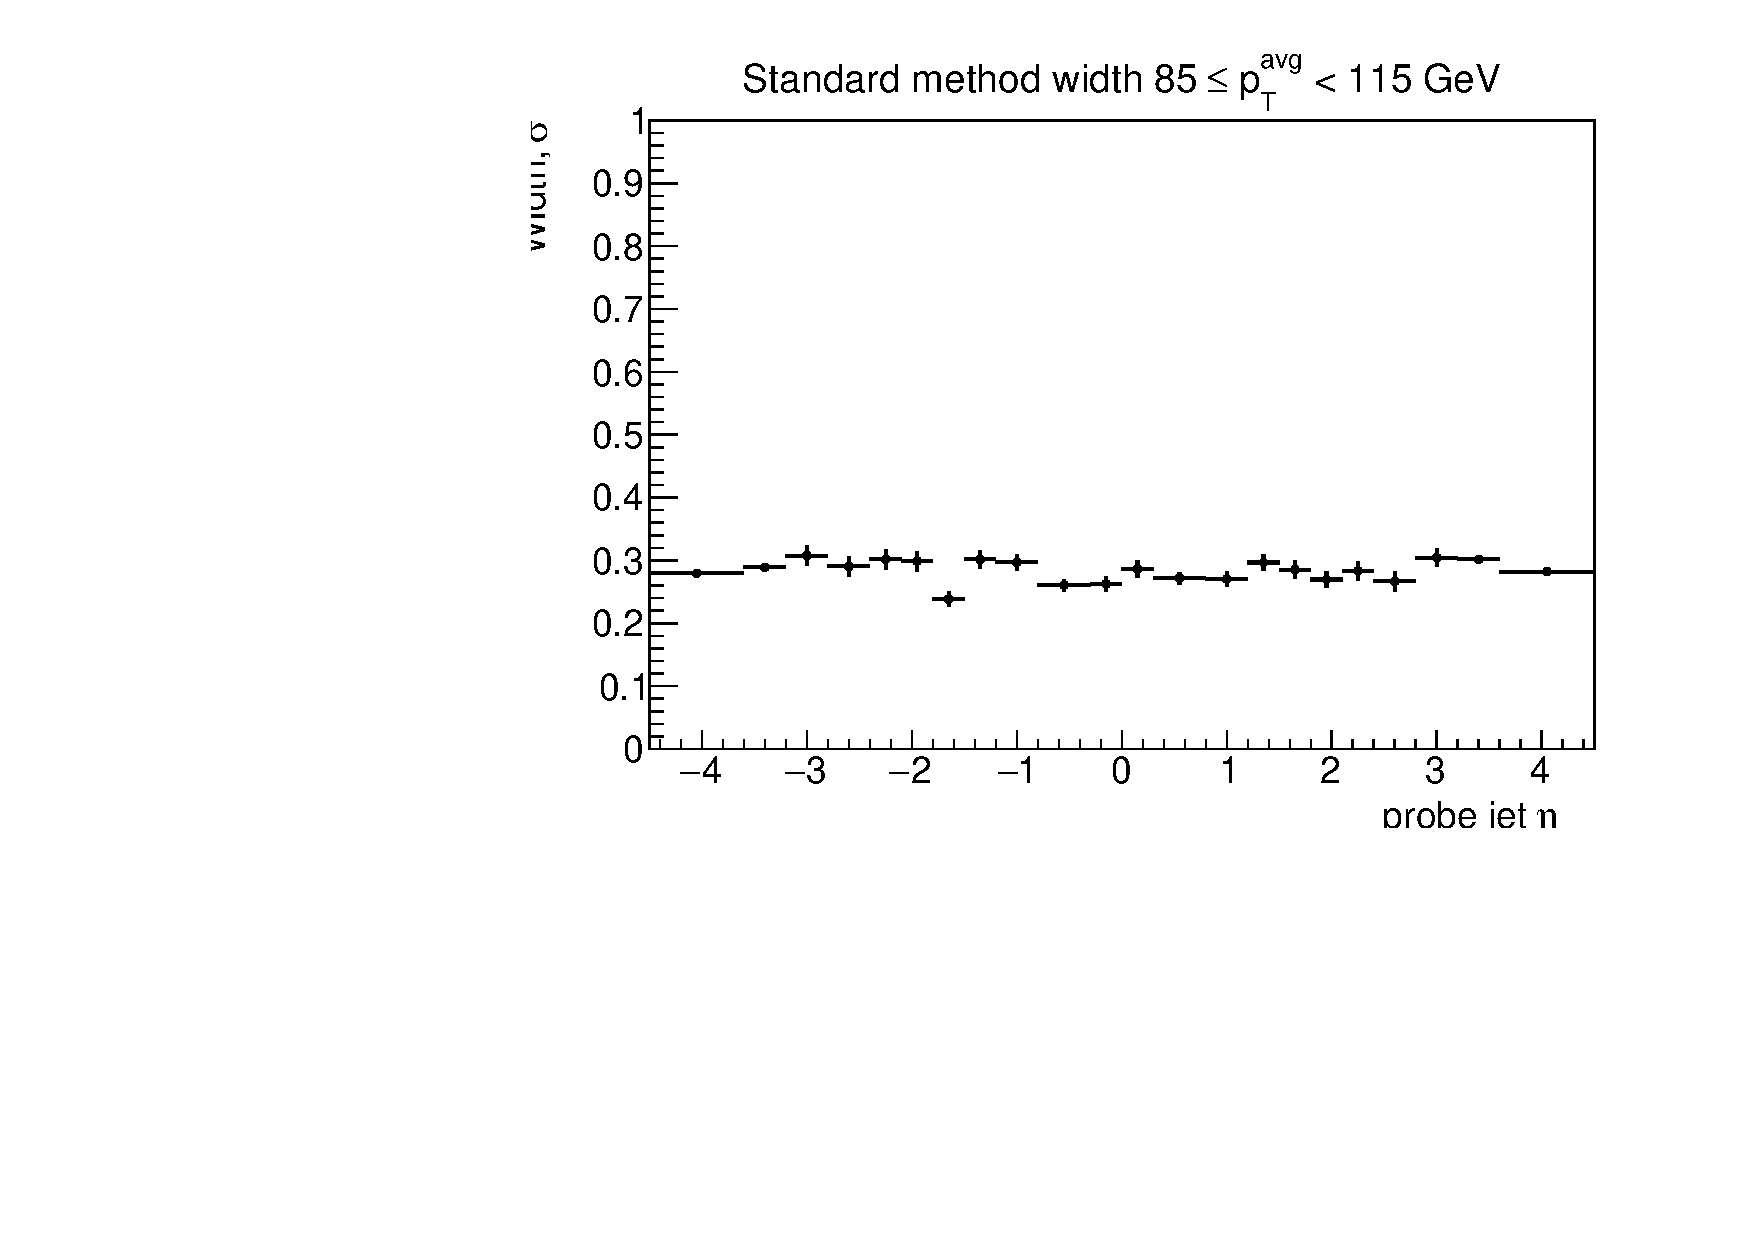
\includegraphics[width=5cm]{Width_vs_ProbeJetEta_85to115GeV_SM.pdf}
\end{column}
\begin{column}{.4\textwidth}
\begin{exampleblock}{Jet Pt Asymmetry Width}
\begin{itemize}
\item Used the fit of the asymmetry of the Pt of jets.
\item Found the Width of this asymmetry.
\end{itemize}
\end{exampleblock}
\end{column}
\end{columns}
\begin{itemize}
\item Then find the Jet Resolution using: $\sigma(A)=\frac{1}{\sqrt{2}}\frac{\sigma(p_{T})}{p_{T}}$
\end{itemize}
\end{frame}

\begin{frame}
\frametitle{Next Steps...}
\begin{itemize}
\item Continue with Jet Energy Resolution Work.
\item Look at DM Phenomenology studies.
\item Prepare for ATLAS DM search for Spring-Summer 2016
\item Expand to look at other new physics signatures in VBF, such as lepton number/flavour violating processes:
\begin{itemize}
\item Heavy Majorana neutrinos
\item Doubly charged Higgs
\item etc.
\end{itemize}
\end{itemize}
\end{frame}

\begin{frame}
\center
\textcolor{red}{\Huge{\textbf{Merry Christmas!}}}
\end{frame}




\end{document} 